% Part: history
% Chapter: set-theory
% Section: limits

\documentclass[../../../include/open-logic-section]{subfiles}

\begin{document}

\olfileid{his}{set}{limits}

\olsection{सीमांची काटेकोर व्याख्या}

आजकाल आधीच्या समस्येवरचे प्रमाणित उत्तर म्हणजे अतिसूक्ष्म राशींचा आधार सोडणे. ते कसे करता येते ते पाहू.

आपण पाहिले की $\beta$ जसजसा लहान होतो तसतशी उताराची अधिक चांगली सन्निकटने मिळतात. खरे तर $\beta$ हा $0$ च्या कितीही जवळ जात असताना, $f'(c)$ या आधीच्या सूत्रातील भागाकाराचा मान आपल्याला हव्या असलेल्या उताराकडे झुकतो. त्यामुळे $\beta = 0$ \emph{असतानाची} स्थिती पाहण्याऐवजी, $\beta$ हा $0$ कडे जात असताना $f'(c)$ च्या त्या सूत्रातील भागाकाराचा \emph{कल} पाहणे पुरेसे आहे.

अशा प्रकारे मांडल्यास, पुढील स्वरूपाच्या विधानांचा अर्थ स्पष्ट करणे हे सर्वसाधारण आव्हान ठरते:
\begin{center}
$x$ हा $c$ कडे जात असताना $g(x)$ चे मूल्य $\ell$ कडे झुकते.
\end{center}
हे अधिक संक्षेपात असे लिहिता येते:
\[
\lim_{x \rightarrow c}g(x) = \ell.
\]
एकोणिसाव्या शतकात कॉशी यांच्या आधीच्या कार्यावर आधार घेत वायेरश्ट्रास यांनी या विधानाची पूर्णपणे काटेकोर व्याख्या दिली. $x$ हा $c$ च्या योग्य इतका जवळ घेतल्यास $g(x)$ हे $\ell$ च्या आपल्याला हवे तितके जवळ नेता येते, हीच त्यामागील कल्पना आहे. अधिक नेमकेपणे, $\lim_{x \rightarrow c} g(x) = \ell$ याचा अर्थ असा ठरवू:
\[
(\forall\epsilon > 0)(\exists \delta > 0)\forall x \left(0 < |x - c| < \delta \lif |g(x) - \ell| < \epsilon \right).
\]
%READERNOTE{OLINC-314: स्रोताच्या सीमा-व्याख्येत x=c वगळलेले नाही; मराठी सूत्रात 0<|x-c| ही आवश्यक अट घातली आहे.}
येथील उभ्या रेषा निरपेक्ष मूल्य दर्शवतात. म्हणजे $x \geq 0$ असेल तेव्हा $|x| = x$, आणि $x < 0$ असेल तेव्हा $|x| =-x$; \emph{त्या} फलनाचा आलेख पुढीलप्रमाणे दाखवता येतो:
\begin{center}
	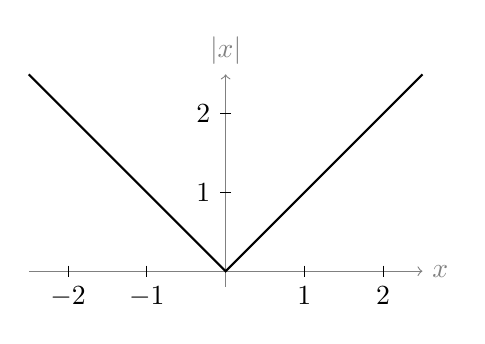
\begin{tikzpicture}[scale=1]
	\draw[->, gray] (-2.5,0) -- (2.5,0) node[right] {$x$};
	\draw[->, gray] (0,-.2) -- (0,2.5) node[above] {$|x|$};

	\foreach \x/\xtext in {-2/-2, -1/-1, 1/1, 2/2}
	\draw[shift={(\x,0)}] (0pt,2pt) -- (0pt,-2pt) node[below] {{$\xtext$}};

	\foreach \y/\ytext in {1/1, 2/2}
	\draw[shift={(0,\y)}] (2pt,0pt) -- (-2pt,0pt) node[left] {{$\ytext$}};

	\draw[thick] (-2.5, 2.5)--(0,0)--(2.5, 2.5);
	\end{tikzpicture}
\end{center}
म्हणून या व्याख्येचा ढोबळ अर्थ असा: $c$ पेक्षा वेगळी पण त्याच्या $\delta$ इतक्या जवळची आदाने निवडून (म्हणजे $0 < |x - c| < \delta$), आपली “त्रुटी” $\epsilon$ पेक्षा लहान करता येते (म्हणजे $|g(x) - \ell| < \epsilon$).

सीमेची संकल्पना व्याख्येने निश्चित केल्यावर आपण अतिसूक्ष्म राशी पूर्णपणे टाळू शकतो. त्यासाठी $c$ येथील $f$ चा उतार असा ठरवू:
\[
	{f}'(c) = \lim_{x \rightarrow 0}\left(\frac{f(c +x) - f(c)}{x}\right) \text{ जेथे सीमा अस्तित्वात आहे}.
\]
मात्र “जेथे सीमा अस्तित्वात आहे” ही अट व्याख्येत का हवी, हे लक्षात घेणे महत्त्वाचे आहे. साधे उदाहरण म्हणून आपण आत्ताच ज्याचा आलेख पाहिला तो $f(x) = |x|$ विचारात घ्या. येथे $f'(0)$ ची व्याख्या होत नाही: $0$ कडे “उजवीकडून” गेल्यास उतार नेहमी $1$ असतो, तर $0$ कडे “डावीकडून” गेल्यास उतार नेहमी $-1$ असतो; म्हणून सीमा अस्तित्वात नाही. त्यामुळे अशी सीमा अस्तित्वात असेल तर आणि तरच फलन~$f$ हे~$x$ येथे \emph{अवकलनीय} आहे, असेही म्हणता येईल.

अवकलनासाठी \emph{सीमेची} संकल्पना कशी वापरायची ते आपण पाहिले. त्याच संकल्पनेने \emph{सतत} फलनाची कल्पनाही व्याख्येने निश्चित करता येते. (१८१७ पर्यंत बोल्झानो यांना हे तत्त्वतः उमगले होते.) कॉशी–वायेरश्ट्रास यांची सातत्याची मांडणी अशी आहे. ढोबळपणे: फलनाच्या निर्गतात ठरावीक अचूकता हवी असेल, तर आदानात पुरेशी अचूकता मागून ती मिळेल, अशा वेळी फलन~$f$ त्या बिंदूवर सतत असते. अधिक नेमकेपणे: $x$ हा शून्याकडे जात असताना $f(c + x)$ आणि $f(c)$ यांतील फरकही $0$ कडे जात असेल, तर $f$ हे $c$ येथे सतत आहे. दुसऱ्या शब्दांत, $f(c) = \lim_{x \rightarrow c} f(x)$ असेल तर आणि तरच $f$ हे $c$ येथे \emph{सतत} आहे.

यापुढे गेलो तर आपला विषय असलेल्या संच उपपत्तीपासून दूर जाऊन आपण वास्तव विश्लेषणात शिरू. म्हणून आता थांबून मुख्य बोध सांगू. एकोणिसाव्या शतकात गणितज्ञांनी काटेकोरपणे व्याख्या केलेल्या \emph{सीमेच्या} संकल्पनेचा वापर करून अतिसूक्ष्म राशींशिवाय काम करायला शिकले.

\end{document}
